\documentclass[10pt]{beamer}
\usepackage{verbatim}
\usepackage{amsmath}
\usepackage{amsthm}
\usepackage{graphics}
\usepackage{color}
\usepackage{algorithm, algorithmic}
\usepackage{stmaryrd}\usefonttheme[onlymath]{serif}

\title{Discussion 3: Algorithm V1 \& Experiment on Cases}
\begin{document}

\maketitle
\begin{frame}\frametitle{Algorithm Version 1}
\begin{algorithm}[H]
\caption{Algorithm Version1: Learn Multiphase RF Incrementally}
\begin{algorithmic}[1]
\REQUIRE Loop $L$, depthBound $db$

\ENSURE $\texttt{result}\in \{\texttt{FIN, INF, UNKNOWN}\}$, a list of RFs \texttt{rf\_list}
\STATE $i := 0, \texttt{result} := \texttt{UNKNOWN},\texttt{rf\_list} := []$
\WHILE{$i < db$ and \texttt{result}$ == \texttt{UNKNOWN}$}
\STATE \texttt{result}, \texttt{rf} $ = $ \texttt{LearnRankerBounded}$(L)$
\IF{$\texttt{result} == \texttt{INF}$ or $\texttt{result} == \texttt{FIN}$}
\STATE $\texttt{rf\_list.append(rf)}$
\STATE $\texttt{return result, rf\_list}$
\ELSE 
\STATE \texttt{result}, \texttt{rf} $ = $ \texttt{LearnRankerNoBound}$(L)$
\STATE \texttt{rf\_list.append(rf)}
\ENDIF
\STATE $L = $ \texttt{ConjunctConstraint($L$, rf)}
\STATE $i \texttt{+=} 1$
\ENDWHILE
\STATE \texttt{return UNKNOWN, rf\_list}
\end{algorithmic}
\end{algorithm}
\end{frame}


\begin{frame}\frametitle{Case 1: Multiphase}
\begin{example}
\texttt{while($x$ > 0 or $y$ > 0) do }$x' = x + y - 1; y' = y - 1$

is a loop ranked by 2-phase multiphase ranking function: $\langle y, x\rangle$
\end{example}

Result of the algorithm: $\langle 0.9971 y, 0.639x + 0.6774\rangle$

\begin{center}
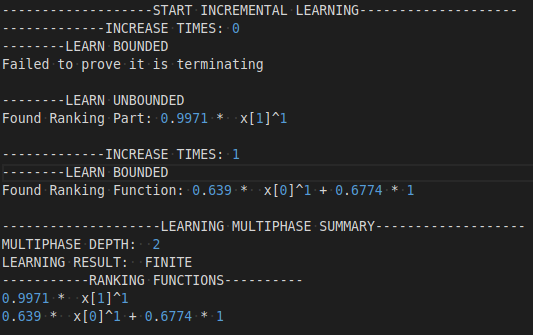
\includegraphics[scale=0.5]{1.png}
\end{center}

\end{frame}

\begin{frame}\frametitle{Case 2: Multiphase plus Branch}
\begin{example}
\texttt{while($x$ > 0 or $y$ > 0) do }

$\texttt{If y > 0:} x' = x; y' = y - 1;$
$\texttt{else:} x' = x - 1; y' = y;$


\end{example}

is a loop with 2-phase multiphase ranking function $\langle y, x\rangle$

Use template $ax + by + c$ to run:
\begin{center}
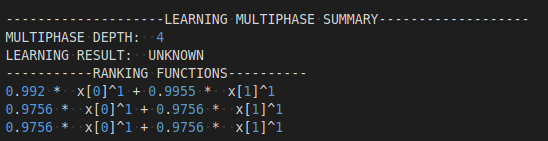
\includegraphics[scale= 0.5]{2.png}
\end{center}
where the learn unbound part always generating $x + y$ as a decreasing function.

\end{frame}

\begin{frame}\frametitle{Way to solve the problem}
Try a different template when learning failed.

If we try $by + c$ as the first template and $ax + by + c$ as the second:

\begin{center}

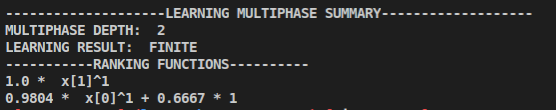
\includegraphics[scale= 0.5]{3.png}
\end{center}

We have to modify our algorithm to by adding back-tracking to try different templates when we fail to learn a ranking function out. 
\end{frame}

\begin{frame}\frametitle{Case 3: Split Technique}
\begin{example}
\texttt{while($x$ > 0 or $y$ > 0) do }$x' = x + y; y' = y - 1$

This is a false example for multiphase ranking function $\langle y,x\rangle$ for when $y < 0$ 
\[ x - x' = -y > 0\]

not $\delta$.



\end{example}

By seting the conjuncted formula to $ y < -0.1$,
 $-y > 0.1$. The multiphase ranking function is $\langle y+0.1, x\rangle$


\end{frame}

\begin{frame}\frametitle{Case 4: Not all cases can be solved}
\begin{example}
\texttt{while($x \ge 1$ and $y \ge 1 $ and $x \ge y$ and $2^By \ge x$) do }$x' = 2x; y' = 3y$

\end{example}
According to "On Multiphase" paper, this loop has a multiphase ranking function:

\[\langle x - 2^By, x - 2^{B-1}y, \ldots, x - y\rangle\]


We ran a experiment on $B = 2$. But failed to learn the RF out.
\begin{center}
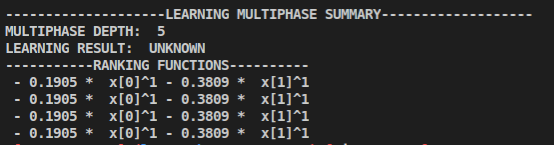
\includegraphics[scale=0.5]{5.png}
\end{center}

Reason: the first guess is incorrect.
\end{frame}



\begin{frame}\frametitle{Algorithm Version 2}

\begin{algorithm}[H]
\caption{Algorithm Version2: Learn Multiphase RF Backtracking }
\begin{algorithmic}[1]
\REQUIRE Loop $L$, depthBound $db$, templateList \texttt{tpList}

\ENSURE $\texttt{result}\in \{\texttt{FIN, INF, UNKNOWN}\}$, a list of RFs \texttt{rf\_list}
\STATE $i = 1$
\WHILE{$i \le db$ and \texttt{result} $==$ \texttt{UNKNOWN}}
\STATE \texttt{rf\_list = []}
\STATE \texttt{result, rf\_list}$=$\texttt{train\_backtracking\_loopbody}($L$, \texttt{rf\_list}, \texttt{tpList}, 0, 1, $i$)
\IF{\texttt{result != UNKNOWN}}
	\textbf{return result, rf\_list}
\ENDIF
\ENDWHILE
\end{algorithmic}
\end{algorithm}

\end{frame}

\begin{frame}\frametitle{Algorithm Version 2 Continue}

\begin{algorithm}[H]
\caption{Algorithm Version2: Learn Multiphase RF Backtracking }
\begin{algorithmic}[1]

\STATE \texttt{train\_backtracking\_loopbody}($L$, \texttt{rf\_list}, \texttt{tpList}, \texttt{tempId}, \texttt{currentDepth}, \texttt{maxDepth}):

\end{algorithmic}
\end{algorithm}

Use dfs to learn multiphase ranking function, if for one layer the learning result is \texttt{UNKNOWN}, backtrack one depth and change the template.
\end{frame}

\begin{frame}\frametitle{Case 5: Jump In-and-Out}
\begin{example}
\texttt{while($x$ > 0 or $y$ > 0) do }

$\texttt{If y > 0:} x' = x; y' = y - 2;$
$\texttt{else:} x' = x - 1; y' = y + 1;$

\end{example}
\begin{itemize}
\item Not backtracking: cannot learn out

\item Backtracking:
\begin{center}
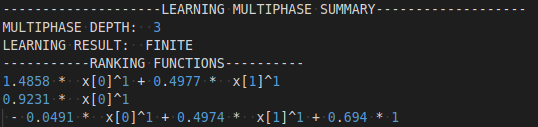
\includegraphics[scale=0.5]{6.png}
\end{center}
\end{itemize}
\end{frame}


\begin{frame}\frametitle{TODOs}
\begin{itemize}

\item Implement the algorithm that extract guard to be the ranking function.

\item Add to deal with nodeterministic loops.

\item Find more cases and explore the advantage of our methods, and do some large scale experiment.
\end{itemize}
\end{frame}

\end{document}